% Options for packages loaded elsewhere
\PassOptionsToPackage{unicode}{hyperref}
\PassOptionsToPackage{hyphens}{url}
\documentclass[
]{article}
\usepackage{xcolor}
\usepackage{amsmath,amssymb}
\setcounter{secnumdepth}{-\maxdimen} % remove section numbering
\usepackage{iftex}
\ifPDFTeX
  \usepackage[T1]{fontenc}
  \usepackage[utf8]{inputenc}
  \usepackage{textcomp} % provide euro and other symbols
\else % if luatex or xetex
  \usepackage{unicode-math} % this also loads fontspec
  \defaultfontfeatures{Scale=MatchLowercase}
  \defaultfontfeatures[\rmfamily]{Ligatures=TeX,Scale=1}
\fi
\usepackage{lmodern}
\ifPDFTeX\else
  % xetex/luatex font selection
\fi
% Use upquote if available, for straight quotes in verbatim environments
\IfFileExists{upquote.sty}{\usepackage{upquote}}{}
\IfFileExists{microtype.sty}{% use microtype if available
  \usepackage[]{microtype}
  \UseMicrotypeSet[protrusion]{basicmath} % disable protrusion for tt fonts
}{}
\makeatletter
\@ifundefined{KOMAClassName}{% if non-KOMA class
  \IfFileExists{parskip.sty}{%
    \usepackage{parskip}
  }{% else
    \setlength{\parindent}{0pt}
    \setlength{\parskip}{6pt plus 2pt minus 1pt}}
}{% if KOMA class
  \KOMAoptions{parskip=half}}
\makeatother
\usepackage{color}
\usepackage{fancyvrb}
\newcommand{\VerbBar}{|}
\newcommand{\VERB}{\Verb[commandchars=\\\{\}]}
\DefineVerbatimEnvironment{Highlighting}{Verbatim}{commandchars=\\\{\}}
% Add ',fontsize=\small' for more characters per line
\newenvironment{Shaded}{}{}
\newcommand{\AlertTok}[1]{\textcolor[rgb]{1.00,0.00,0.00}{\textbf{#1}}}
\newcommand{\AnnotationTok}[1]{\textcolor[rgb]{0.38,0.63,0.69}{\textbf{\textit{#1}}}}
\newcommand{\AttributeTok}[1]{\textcolor[rgb]{0.49,0.56,0.16}{#1}}
\newcommand{\BaseNTok}[1]{\textcolor[rgb]{0.25,0.63,0.44}{#1}}
\newcommand{\BuiltInTok}[1]{\textcolor[rgb]{0.00,0.50,0.00}{#1}}
\newcommand{\CharTok}[1]{\textcolor[rgb]{0.25,0.44,0.63}{#1}}
\newcommand{\CommentTok}[1]{\textcolor[rgb]{0.38,0.63,0.69}{\textit{#1}}}
\newcommand{\CommentVarTok}[1]{\textcolor[rgb]{0.38,0.63,0.69}{\textbf{\textit{#1}}}}
\newcommand{\ConstantTok}[1]{\textcolor[rgb]{0.53,0.00,0.00}{#1}}
\newcommand{\ControlFlowTok}[1]{\textcolor[rgb]{0.00,0.44,0.13}{\textbf{#1}}}
\newcommand{\DataTypeTok}[1]{\textcolor[rgb]{0.56,0.13,0.00}{#1}}
\newcommand{\DecValTok}[1]{\textcolor[rgb]{0.25,0.63,0.44}{#1}}
\newcommand{\DocumentationTok}[1]{\textcolor[rgb]{0.73,0.13,0.13}{\textit{#1}}}
\newcommand{\ErrorTok}[1]{\textcolor[rgb]{1.00,0.00,0.00}{\textbf{#1}}}
\newcommand{\ExtensionTok}[1]{#1}
\newcommand{\FloatTok}[1]{\textcolor[rgb]{0.25,0.63,0.44}{#1}}
\newcommand{\FunctionTok}[1]{\textcolor[rgb]{0.02,0.16,0.49}{#1}}
\newcommand{\ImportTok}[1]{\textcolor[rgb]{0.00,0.50,0.00}{\textbf{#1}}}
\newcommand{\InformationTok}[1]{\textcolor[rgb]{0.38,0.63,0.69}{\textbf{\textit{#1}}}}
\newcommand{\KeywordTok}[1]{\textcolor[rgb]{0.00,0.44,0.13}{\textbf{#1}}}
\newcommand{\NormalTok}[1]{#1}
\newcommand{\OperatorTok}[1]{\textcolor[rgb]{0.40,0.40,0.40}{#1}}
\newcommand{\OtherTok}[1]{\textcolor[rgb]{0.00,0.44,0.13}{#1}}
\newcommand{\PreprocessorTok}[1]{\textcolor[rgb]{0.74,0.48,0.00}{#1}}
\newcommand{\RegionMarkerTok}[1]{#1}
\newcommand{\SpecialCharTok}[1]{\textcolor[rgb]{0.25,0.44,0.63}{#1}}
\newcommand{\SpecialStringTok}[1]{\textcolor[rgb]{0.73,0.40,0.53}{#1}}
\newcommand{\StringTok}[1]{\textcolor[rgb]{0.25,0.44,0.63}{#1}}
\newcommand{\VariableTok}[1]{\textcolor[rgb]{0.10,0.09,0.49}{#1}}
\newcommand{\VerbatimStringTok}[1]{\textcolor[rgb]{0.25,0.44,0.63}{#1}}
\newcommand{\WarningTok}[1]{\textcolor[rgb]{0.38,0.63,0.69}{\textbf{\textit{#1}}}}
\usepackage{longtable,booktabs,array}
\usepackage{caption}
\captionsetup[table]{skip=6pt}
\newcounter{none} % for unnumbered tables
\usepackage{calc} % for calculating minipage widths
% Correct order of tables after \paragraph or \subparagraph
\usepackage{etoolbox}
\makeatletter
\patchcmd\longtable{\par}{\if@noskipsec\mbox{}\fi\par}{}{}
\makeatother
% Allow footnotes in longtable head/foot
\IfFileExists{footnotehyper.sty}{\usepackage{footnotehyper}}{\usepackage{footnote}}
\makesavenoteenv{longtable}
\usepackage{graphicx}
\makeatletter
\newsavebox\pandoc@box
\newcommand*\pandocbounded[1]{% scales image to fit in text height/width
  \sbox\pandoc@box{#1}%
  \Gscale@div\@tempa{\textheight}{\dimexpr\ht\pandoc@box+\dp\pandoc@box\relax}%
  \Gscale@div\@tempb{\linewidth}{\wd\pandoc@box}%
  \ifdim\@tempb\p@<\@tempa\p@\let\@tempa\@tempb\fi% select the smaller of both
  \ifdim\@tempa\p@<\p@\scalebox{\@tempa}{\usebox\pandoc@box}%
  \else\usebox{\pandoc@box}%
  \fi%
}
% Set default figure placement to htbp
\def\fps@figure{htbp}
\makeatother
\ifLuaTeX
  \usepackage{luacolor}
  \usepackage[soul]{lua-ul}
\else
  \usepackage{soul}
\fi
% definitions for citeproc citations
\NewDocumentCommand\citeproctext{}{}
\NewDocumentCommand\citeproc{mm}{%
  \begingroup\def\citeproctext{#2}\cite{#1}\endgroup}
\makeatletter
 % allow citations to break across lines
 \let\@cite@ofmt\@firstofone
 % avoid brackets around text for \cite:
 \def\@biblabel#1{}
 \def\@cite#1#2{{#1\if@tempswa , #2\fi}}
\makeatother
\newlength{\cslhangindent}
\setlength{\cslhangindent}{1.5em}
\newlength{\csllabelwidth}
\setlength{\csllabelwidth}{3em}
\newenvironment{CSLReferences}[2] % #1 hanging-indent, #2 entry-spacing
 {\begin{list}{}{%
  \setlength{\itemindent}{0pt}
  \setlength{\leftmargin}{0pt}
  \setlength{\parsep}{0pt}
  % turn on hanging indent if param 1 is 1
  \ifodd #1
   \setlength{\leftmargin}{\cslhangindent}
   \setlength{\itemindent}{-1\cslhangindent}
  \fi
  % set entry spacing
  \setlength{\itemsep}{#2\baselineskip}}}
 {\end{list}}
\usepackage{calc}
\newcommand{\CSLBlock}[1]{\hfill\break\parbox[t]{\linewidth}{\strut\ignorespaces#1\strut}}
\newcommand{\CSLLeftMargin}[1]{\parbox[t]{\csllabelwidth}{\strut#1\strut}}
\newcommand{\CSLRightInline}[1]{\parbox[t]{\linewidth - \csllabelwidth}{\strut#1\strut}}
\newcommand{\CSLIndent}[1]{\hspace{\cslhangindent}#1}
\setlength{\emergencystretch}{3em} % prevent overfull lines
\providecommand{\tightlist}{%
  \setlength{\itemsep}{0pt}\setlength{\parskip}{0pt}}
\makeatletter
\@ifpackageloaded{subcaption}{}{\usepackage{subcaption}}
\@ifpackageloaded{caption}{}{\usepackage{caption}}
\captionsetup[subfigure]{margin=0.5em}
\AtBeginDocument{%
\renewcommand*\figurename{Figure}
\renewcommand*\tablename{Table}
}
\AtBeginDocument{%
\renewcommand*\listfigurename{List of Figures}
\renewcommand*\listtablename{List of Tables}
}
\newcounter{pandoccrossref@subfigures@footnote@counter}
\newenvironment{pandoccrossrefsubfigures}{%
\setcounter{pandoccrossref@subfigures@footnote@counter}{0}
\begin{figure}\centering%
\gdef\global@pandoccrossref@subfigures@footnotes{}%
\DeclareRobustCommand{\footnote}[1]{\footnotemark%
\stepcounter{pandoccrossref@subfigures@footnote@counter}%
\ifx\global@pandoccrossref@subfigures@footnotes\empty%
\gdef\global@pandoccrossref@subfigures@footnotes{{##1}}%
\else%
\g@addto@macro\global@pandoccrossref@subfigures@footnotes{, {##1}}%
\fi}}%
{\end{figure}%
\addtocounter{footnote}{-\value{pandoccrossref@subfigures@footnote@counter}}
\@for\f:=\global@pandoccrossref@subfigures@footnotes\do{\stepcounter{footnote}\footnotetext{\f}}%
\gdef\global@pandoccrossref@subfigures@footnotes{}}
\@ifpackageloaded{float}{}{\usepackage{float}}
\floatstyle{ruled}
\@ifundefined{c@chapter}{\newfloat{codelisting}{h}{lop}}{\newfloat{codelisting}{h}{lop}[chapter]}
\floatname{codelisting}{Listing}
\newcommand*\listoflistings{\listof{codelisting}{List of Listings}}
\makeatother
\usepackage{bookmark}
\IfFileExists{xurl.sty}{\usepackage{xurl}}{} % add URL line breaks if available
\urlstyle{same}
% fallback for those not using the hyperref driver hyperxmp:
\makeatletter
\@ifundefined{xmpquote}{\newcommand{\xmpquote}[1]{#1}}{}
\makeatother
\hypersetup{
  pdftitle={Pandoc check: title block{,} cross-references and captions},
  pdfauthor={Ada Lovelace, University of London; Charles Babbage, University of Cambridge; Mary Somerville},
  hidelinks,
  pdfcreator={LaTeX via pandoc}}

\title{Pandoc check: title block, cross-references and captions}
\author{Ada Lovelace, University of London \and Charles Babbage,
University of Cambridge \and Mary Somerville}
\date{27 October 2026}

\begin{document}
\maketitle
\begin{abstract}
This document checks what Word and LaTeX receive from Halmos. The
abstract cites a source {[}1{]}, has \emph{emphasis} and an inline
formula \(E = mc^2\), and refers to \textbf{fig:photo?}.
\end{abstract}

Each section opens with a \textbf{Check:} line saying what the Word
(\texttt{.docx}) and LaTeX (\texttt{.tex}) output should show. Export
this file to PDF, Word and LaTeX, and compare. The style is IEEE, so
citations are numbered in reading order.

\subsection{1. Title block}\label{title-block}

\textbf{Check:} - \textbf{Title:} shown once, with its colon kept. -
\textbf{Authors:} all three appear. In Word and LaTeX, the first two
read ``Ada Lovelace, University of London'' and ``Charles Babbage,
University of Cambridge'', and the third reads ``Mary Somerville''. -
\textbf{Date:} ``27 October 2026'', exactly as written. -
\textbf{Abstract:} - It shows its italic word and its formula. - Its
citation is {[}1{]}, the first number in the document. - Its reference
reads ``Figure 1''. - \textbf{PDF:} no header on page 1. From page 2,
the title is at the top of each page, and ``Page N of M'' is at the
bottom of every page. - \textbf{Word and LaTeX:} no stray
\texttt{\{title\}} or ``Page \{page\}'' text anywhere.

\subsection{2. Text}\label{text}

\textbf{Check:} - Bold, italic, strike-through, inline code and the link
all survive. - Both footnotes are numbered and listed at the end (Word)
or at the foot of the page (LaTeX).

This line has \textbf{bold}, \emph{italic}, \st{struck} and
\texttt{inline\ code}, and a \href{https://pandoc.org}{link to Pandoc}.
A first footnote\footnote{The first note, with a formula
  \(a^2 + b^2 = c^2\).} and a second\footnote{The second note, citing
  {[}2{]}.}.

\begin{quote}
A block quotation, which should be indented in every format.
\end{quote}

\subsection{3. Lists}\label{lists}

\textbf{Check:} - \textbf{Nesting:} both lists keep their nesting. -
\textbf{Numbering:} the numbered list counts 1, 2, 3. - \textbf{Task
list:} shows ticked and empty boxes, or plain bullets, but never
\texttt{{[}\ {]}} as text.

\begin{itemize}
\tightlist
\item
  First point

  \begin{itemize}
  \tightlist
  \item
    Nested point
  \item
    Another nested point
  \end{itemize}
\item
  Second point
\end{itemize}

\begin{enumerate}
\def\labelenumi{\arabic{enumi}.}
\tightlist
\item
  Step one
\item
  Step two

  \begin{enumerate}
  \def\labelenumii{\arabic{enumii}.}
  \tightlist
  \item
    Sub-step
  \end{enumerate}
\item
  Step three
\end{enumerate}

\begin{itemize}
\tightlist
\item[$\boxtimes$]
  A finished task
\item[$\square$]
  An open task
\end{itemize}

\subsection{4. Citations}\label{citations}

\textbf{Check:} - Every form below formats in IEEE style. - Numbers
continue from the abstract's {[}1{]}. - The unknown key shows as
``(nosuch2099?)'' in Word and LaTeX, as Pandoc does. - \textbf{Reference
list:} comes after the text under a ``References'' heading that Halmos
adds, so the document doesn't write one. It's in IEEE order and leaves
out the unknown key.

\begin{itemize}
\tightlist
\item
  One source {[}3{]}.
\item
  Two at once {[}4{]}, {[}5{]}.
\item
  Narrative: {[}6{]} shows this.
\item
  With a page: see {[}2, p. 3{]}.
\item
  Year only: {[}1{]}.
\item
  Unknown key: \textbf{nosuch2099?}.
\end{itemize}

\subsection{5. Figures}\label{figures}

\textbf{Check:} - \textbf{Numbering:} the figures are numbered 1, 2, 3,
4 in this order in every format, with captions such as ``Figure 1:
\ldots{}''. - \textbf{Images:} the decorative image has no number and no
caption. - \textbf{Charts and diagrams:} - Word: the chart and the
diagram are pictures. - LaTeX: they stay as code, so they are not
figures there. This is known.

A labelled image:

\begin{figure}
\centering
\pandocbounded{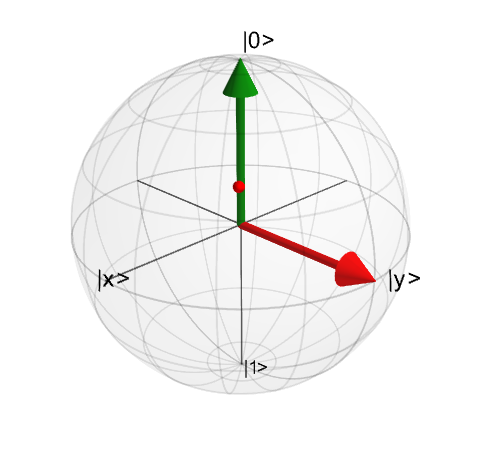
\includegraphics[keepaspectratio,alt={A labelled photograph}]{images/pasted-20261018-130949.png}}
\caption{A labelled photograph}\label{fig:photo}
\end{figure}

An unlabelled captioned image. Halmos gives it a hidden label for
export, so it is still numbered:

\begin{figure}
\centering
\pandocbounded{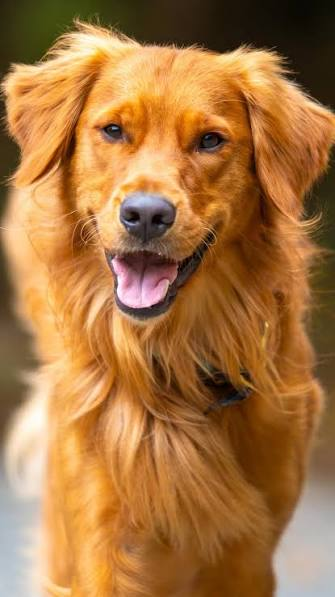
\includegraphics[keepaspectratio,alt={An unlabelled photograph}]{images/pasted-20261018-134231.png}}
\caption{An unlabelled photograph}\label{fig:halmos-1}
\end{figure}

A decorative image, with no alt text:

\pandocbounded{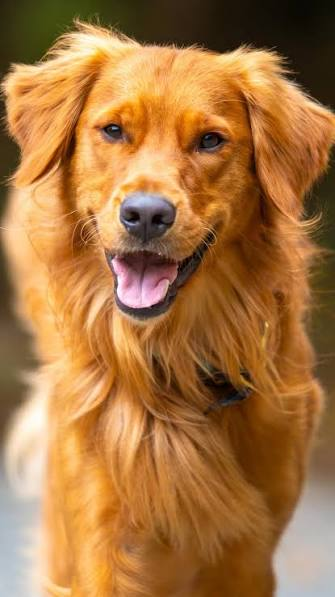
\includegraphics[keepaspectratio]{images/pasted-20261018-134353.png}}

A labelled chart:

\protect\phantomsection\label{fig:chart}%
\begin{Shaded}
\begin{Highlighting}[]
\NormalTok{\{}
\NormalTok{  "title": "Recovered sources by category",}
\NormalTok{  "data": \{"values": [}
\NormalTok{    \{"category": "A", "value": 12\}, \{"category": "B", "value": 27\},}
\NormalTok{    \{"category": "C", "value": 19\}}
\NormalTok{  ]\},}
\NormalTok{  "mark": "bar",}
\NormalTok{  "encoding": \{}
\NormalTok{    "x": \{"field": "category", "type": "nominal"\},}
\NormalTok{    "y": \{"field": "value", "type": "quantitative"\}}
\NormalTok{  \}}
\NormalTok{\}}
\end{Highlighting}
\end{Shaded}

A labelled diagram:

\protect\phantomsection\label{fig:pipeline}%
\begin{Shaded}
\begin{Highlighting}[]
\NormalTok{{-}{-}{-}}
\NormalTok{title: Conversion pipeline}
\NormalTok{{-}{-}{-}}
\NormalTok{flowchart LR}
\NormalTok{  A[Markdown] {-}{-}\textgreater{} B[Halmos export copy]}
\NormalTok{  B {-}{-}\textgreater{} C[Pandoc]}
\NormalTok{  C {-}{-}\textgreater{} D[Word or LaTeX]}
\end{Highlighting}
\end{Shaded}

\subsection{6. Tables}\label{tables}

\textbf{Check:} - \textbf{Numbering:} the two captioned tables are
numbered 1 and 2, apart from the figures. - \textbf{Captions:} each
caption reads ``Table N: \ldots{}'', above its table. -
\textbf{Uncaptioned table:} it has no number. - \textbf{Alignment:}
right-aligned columns stay right-aligned.

\begin{longtable}[]{@{}lrr@{}}
\caption{Yield by treatment}\label{tbl:yield}\tabularnewline
\toprule\noalign{}
Group & Yield (t/ha) & Change \\
\midrule\noalign{}
\endfirsthead
\toprule\noalign{}
Group & Yield (t/ha) & Change \\
\midrule\noalign{}
\endhead
\bottomrule\noalign{}
\endlastfoot
Control & 6.12 & --- \\
Late N & 6.61 & +8\% \\
Split N & 6.48 & +6\% \\
\end{longtable}

\begin{longtable}[]{@{}lr@{}}
\caption{Rainfall by season, with no
label}\label{tbl:halmos-1}\tabularnewline
\toprule\noalign{}
Season & Rainfall (mm) \\
\midrule\noalign{}
\endfirsthead
\toprule\noalign{}
Season & Rainfall (mm) \\
\midrule\noalign{}
\endhead
\bottomrule\noalign{}
\endlastfoot
2024 & 512 \\
2025 & 438 \\
\end{longtable}

{\def\LTcaptype{none} % do not increment counter
\begin{longtable}[]{@{}lll@{}}
\toprule\noalign{}
An & uncaptioned & table \\
\midrule\noalign{}
\endhead
\bottomrule\noalign{}
\endlastfoot
1 & 2 & 3 \\
\end{longtable}
}

\subsection{7. Equations}\label{equations}

\textbf{Check:} - \textbf{Labelled equation:} shows the number (1) at
the right. - \textbf{Unlabelled display equation:} has no number. -
\textbf{Inline maths:} stays in the line.

A labelled equation:

\begin{equation}\protect\phantomsection\label{eq:energy}{ E = mc^2 }\end{equation}

An unlabelled display equation, not numbered:

\[
\int_0^\infty e^{-x^2}\,dx = \frac{\sqrt{\pi}}{2}
\]

Inline: the mean is \(\bar{x} = \tfrac{1}{n}\sum_i x_i\).

\subsection{8. Cross-references}\label{cross-references}

\textbf{Check:} - \textbf{Word:} each reference is linked text, for
example ``Figure 1'' or ``Table 1''. - \textbf{LaTeX:} the references to
the photograph, the table and the equation resolve. The ones to the
chart and the diagram do not, which is known. - \textbf{Missing label:}
the reference to it is visibly broken in every format.

\begin{itemize}
\tightlist
\item
  The labelled photograph: Figure~\ref{fig:photo}.
\item
  At the start of a sentence: Figure~\ref{fig:chart} shows the
  categories.
\item
  Two at once: Figures~\ref{fig:photo}, \ref{fig:pipeline}.
\item
  The table: Table~\ref{tbl:yield}.
\item
  The equation: Equation~\ref{eq:energy}.
\item
  A missing label: Figure~\ref{fig:nosuch}.
\end{itemize}

\subsection{9. Code}\label{code}

\textbf{Check:} - The block keeps its line breaks and indentation, in a
fixed-width font. - Word may colour the syntax; LaTeX may not.

\begin{Shaded}
\begin{Highlighting}[]
\KeywordTok{def}\NormalTok{ mean(xs):}
    \CommentTok{"""The arithmetic mean."""}
    \ControlFlowTok{return} \BuiltInTok{sum}\NormalTok{(xs) }\OperatorTok{/} \BuiltInTok{len}\NormalTok{(xs)}
\end{Highlighting}
\end{Shaded}

\subsection{10. Alerts}\label{alerts}

\textbf{Check:} - GitHub-style alerts have no Pandoc equivalent. Expect
a block quotation that starts with ``{[}!NOTE{]}'' or ``Note''. Record
which one you get.

\begin{quote}
{[}!NOTE{]} An alert, for comparison with the preview.
\end{quote}

\subsection*{References}\label{references}
\addcontentsline{toc}{subsection}{References}

\protect\phantomsection\label{refs}
\begin{CSLReferences}{0}{0}
\bibitem[\citeproctext]{ref-feinQuantumSuperpositionMolecules2019}
\CSLLeftMargin{{[}1{]} }%
\CSLRightInline{Y. Y. Fein \emph{et al.}, {``Quantum superposition of
molecules beyond 25 {kDa},''} \emph{Nature Physics}, vol. 15, no. 12,
pp. 1242--1245, Dec. 2019, doi:
\href{https://doi.org/10.1038/s41567-019-0663-9}{10.1038/s41567-019-0663-9}.}

\bibitem[\citeproctext]{ref-bandiComprehensiveOverviewAtomic2023}
\CSLLeftMargin{{[}2{]} }%
\CSLRightInline{T. N. Bandi, {``A {Comprehensive Overview} of {Atomic
Clocks} and their {Applications},''} \emph{Biology, Engineering,
Medicine and Science Reports}, vol. 9, no. 1, pp. 01--10, Jan. 2023,
doi: \href{https://doi.org/10.5530/bems.9.1.1}{10.5530/bems.9.1.1}.}

\bibitem[\citeproctext]{ref-brackerFineStructureOptical2008}
\CSLLeftMargin{{[}3{]} }%
\CSLRightInline{A. S. Bracker, D. Gammon, and V. L. Korenev, {``Fine
structure and optical pumping of spins in individual semiconductor
quantum dots,''} \emph{Semiconductor Science and Technology}, vol. 23,
no. 11, p. 114004, Nov. 2008, doi:
\href{https://doi.org/10.1088/0268-1242/23/11/114004}{10.1088/0268-1242/23/11/114004}.}

\bibitem[\citeproctext]{ref-branczykHongOuMandelInterference2024}
\CSLLeftMargin{{[}4{]} }%
\CSLRightInline{A. M. Brańczyk, {``Hong-{Ou-Mandel Interference},''}
\emph{Canadian Journal of Physics}, vol. 102, no. 8, pp. 411--421, Aug.
2024, doi:
\href{https://doi.org/10.1139/cjp-2023-0312}{10.1139/cjp-2023-0312}.}

\bibitem[\citeproctext]{ref-coishNuclearSpinsNanostructures2009}
\CSLLeftMargin{{[}5{]} }%
\CSLRightInline{W. A. Coish and J. Baugh, {``Nuclear spins in
nanostructures,''} \emph{physica status solidi (b)}, vol. 246, no. 10,
pp. 2203--2215, Oct. 2009, doi:
\href{https://doi.org/10.1002/pssb.200945229}{10.1002/pssb.200945229}.}

\bibitem[\citeproctext]{ref-DecoherenceQuantumToClassicalTransition2007}
\CSLLeftMargin{{[}6{]} }%
\CSLRightInline{\emph{Decoherence and the {Quantum-To-Classical
Transition}}. in Frontiers {Collection}. Berlin, Heidelberg: Springer
Berlin Heidelberg, 2007. doi:
\href{https://doi.org/10.1007/978-3-540-35775-9}{10.1007/978-3-540-35775-9}.}

\end{CSLReferences}

\end{document}
